\problemname{\problemyamlname}
It is the day before the NWERC and you and your team are on the train towards Delft.
The journey is long and boring but you came up with a good idea: ``Let's do some \emph{train}ing''.

\quad\emph{-- silence --}

You take your laptop out and try to plug it in when you notice that the only socket is already in use.
Your friends smirk and reply: ``No socket for you, no \emph{train}ing for us''.
% His smirk quickly fades as you pull out a power strip, unplug his charger, and plug it back into the power strip.
Their smirks quickly fade as you pull out a power strip, unplug the charger from the socket, and plug it back into the power strip.
Now, there is enough space for your charger as well.
% He obviously did not expect you to be prepared for this\dots
% and plugged his device and your laptop into the power strip.


\begin{figure}[h]
    \centering
    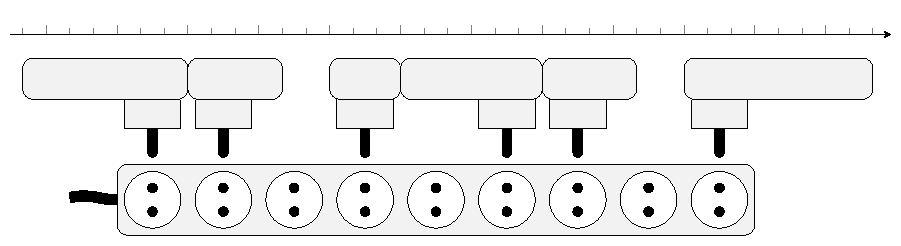
\includegraphics{powerstrip.pdf}
    \caption{
        Illustration of Sample Input 2.
        The first six chargers can be plugged in as shown.
        Note that this is not the only possible solution.
        However, it can be shown that it is impossible to plug in all seven chargers.
    }
    \label{fig:powerstrip}
\end{figure}

However, as soon as more sockets are available, your friends suddenly take out more devices that need to be charged.
You realize that you will not get them to train like this, so you decide to trick them into solving a problem instead.

Your power strip comprises a row of $s$ sockets, and each socket is $\SI{3}{\cm}$ in diameter.
Furthermore, as you examine the chargers, you notice that they all have integer lengths.
The plug of each charger is always on one of the two ends, and each charger can
only be used in two orientations. Chargers cannot overlap, but can touch,
and can extend beyond the end of the power strip as long as they are plugged in
to a socket.
% Given that the part to plug in is always at the outer side of a plug and that you can only plug it in in two orientations
Now you challenge them to charge as many devices as possible.
This is visualized in Figure~\ref{fig:powerstrip}.
Hoping that this allows them to avoid the \emph{train}ing, your friends agree to write a program to solve this.

\begin{Input}
The input consists of:
\begin{itemize}
\item
One line with two integers $n$ and $s$ $(1\leq n\leq2\cdot 10^5$,  $1\leq s\leq10^9)$, the number of chargers you have and the number of sockets on the power strip.
\item
One line with $n$ integers $w$ ($3\leq w\leq10^9$),
the width of each charger in centimetres.
\end{itemize}
Note that you are allowed to rotate chargers by $180^\circ$ before plugging them in.
\end{Input}

\begin{Output}
Output the maximum number of chargers you can plug into the power strip at the same time.
\end{Output}
